\documentclass[12pt]{extarticle}
\usepackage[utf8]{inputenc}
\usepackage{cite}
\usepackage{graphicx}
\usepackage{pdfpages}


\renewcommand{\baselinestretch}{1.25} % for line spacing

\title{Proposal of Website Development for AndE Mamma}
\author{{Adarash Technologies}}
\date{Oct 2022}


\begin{document}

\begin{titlepage}
    \centering
    \vfill
    {\bfseries\Large
        Project Report\\
        for\\
        Tropical Poultry Genetic Solutions (TPGS) Project - Platforms\\
        \vskip2cm
 
    }    
    \vfill
    \vfill 
    \vfill 
    \vspace{15pt}
    \textbf{
    Simon Belete,
    \\
			May 15, 2022 G.C
		}
    
    \vfill
\end{titlepage}

\newpage

\tableofcontents
\newpage

\pagenumbering{arabic}

\section{Nutrition Eduction}
\subsection{Overview}
Nutrition Education Mobile App in three languages(Amharic, English and Swahili), mobile application and the website(additional requirement) are done. The remaining works are content revision and deployment to Play store. 

\subsection{Milestones and Deliverables}
\begin{center}
\begin{tabular}{ |p{7cm}|p{3cm}|p{4cm}| } 
\hline
\textbf{Milestone / Deliverable Name} & \textbf{Status} & \textbf{Remark}  \\
\hline
Develop Mobile Application &  Done &  \\
\hline
Testing Mobile Application &  Ongoing & \\
\hline
Deploy to Play Store &  Ongoing & \\
\hline
\end{tabular}
\end{center}

\subsection{Scope Changes}
Scope changes are requests made by the team that are not stated in the initial Term of Reference(TOR).
\begin{center}
\begin{tabular}{ |p{2cm}|p{7cm}|p{3cm}|p{2cm}| } 
\hline
\textbf{Catagory} & \textbf{Description} & \textbf{Status} & \textbf{Remark}  \\
\hline
Platform & Developing additional Website with the mobile application & Done & \\
\hline

\hline
\end{tabular}
\end{center}

\section{Breeding Data Management}

\subsection{Overview}
Based on the TOR agreement the requested platform was a Mobile Application, but When the mobile application was in beta testing I was requested to develop(change) the platform to a website. Currently the status of the project in 90\%, the remaining works are further development, testing and deployment.

\subsection{Milestones and Deliverables}
\begin{center}
\begin{tabular}{ |p{7cm}|p{3cm}|p{4cm}| } 
\hline
\textbf{Milestone / Deliverable Name} & \textbf{Status} & \textbf{Remark}  \\
\hline
Develop Mobile Application &  Done & Discontinued in beta stage \\
\hline
Testing Mobile Application &  Discontinued & \\
\hline
Deploy to Play Store &  Discontinued & \\
\hline
\end{tabular}
\end{center}

\subsection{Scope Changes}
Scope changes are requests made by the team that are not stated in the initial Term of Reference(TOR).
\begin{center}
\begin{tabular}{ |p{2cm}|p{7cm}|p{3cm}|p{2cm}| } 
\hline
\textbf{Catagory} & \textbf{Description} & \textbf{Status} & \textbf{Remark}  \\
\hline
Platform & Change to a website & Done & 90\% progress \\
\hline
Platform & Deploy to ILRI server & Ongoing & \\
\hline
\end{tabular}
\end{center}

\section{Feed Formulation}

\subsection{Overview}
Based on the TOR agreement the requested platform was a Mobile Application, but requested to be changed into a Website. Currently the status of the project in 95\%, the remaining works are further developments, testing and deployment.

\subsection{Milestones and Deliverables}
\begin{center}
\begin{tabular}{ |p{7cm}|p{3cm}|p{4cm}| } 
\hline
\textbf{Milestone / Deliverable Name} & \textbf{Status} & \textbf{Remark}  \\
\hline
Develop Mobile Application &  Done & 95\% \\
\hline
Testing Mobile Application &  OnGoing & \\
\hline
Deploy to Play Store &  Discontinued & \\
\hline
\end{tabular}
\end{center}

\subsection{Scope Changes}
Scope changes are requests made by the team that are not stated in the initial Term of Reference(TOR).
\begin{center}
\begin{tabular}{ |p{2cm}|p{7cm}|p{3cm}|p{2cm}| } 
\hline
\textbf{Catagory} & \textbf{Description} & \textbf{Status} & \textbf{Remark}  \\
\hline
Platform & Change to a website & Done & 90\% progress \\
\hline
Platform & Deploy to ILRI server & Ongoing & \\
\hline
\end{tabular}
\end{center}

\section{Livestock extension agent training mobile app}
Due to the lack of sufficient time the mobile application development has not been started, the current state of is in information gathering state.

\section{Challenges}
\begin{itemize}
	\item Changes in requirements
	\item Lack of adequate and enough resources in a timely manner 
	\item Lack of Swahili translator
\end{itemize}

\newpage
\section{Remaining Work}

\begin{itemize}
	\item Educational Material content revision
	\item Portal development - A webiste that connect all the applications as one entity
	\item Complete remaining requirements (i.e Technical requirements)
	\begin{itemize}
		\item Improve Website preformance
		\item Search engine optimization
		\item Multi Farm management 
		\item Single sign on(one login crediential Single login credential for all applications)
		\item etc... (Can be stated on request)
	\end{itemize}
	\item Testing applications
	\item Integration testing
	\item Deploy all applications on the ILRI server
\end{itemize}

\section{Refrence}
\begin{figure}[ht]
\centering
%\vspace*{-8cm}
\hspace*{-3cm}
%\noindent
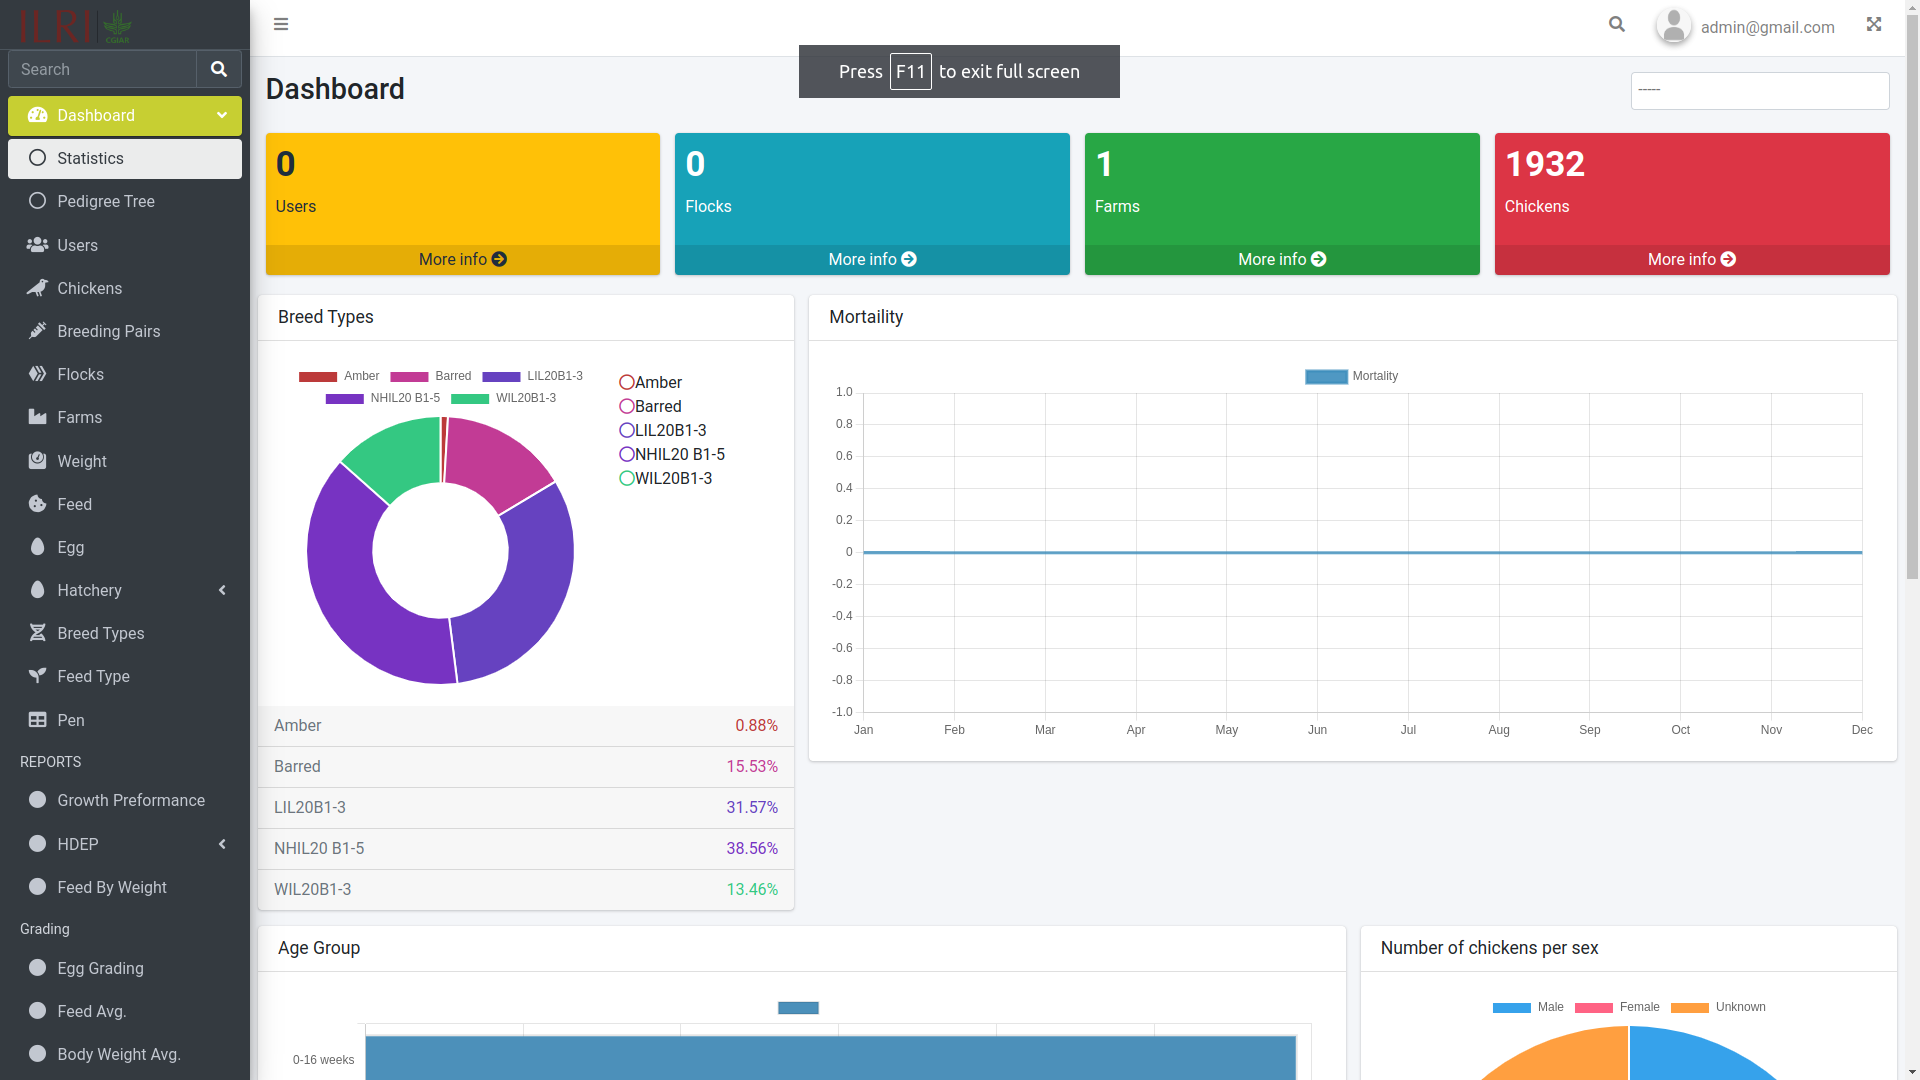
\includegraphics[width=20cm,keepaspectratio]{2.png}
\caption{Breeding Data management dahsbaord}
\end{figure}

\begin{figure}[!ht]
\centering
%\vspace*{-8cm}
\hspace*{-3cm}
%\noindent
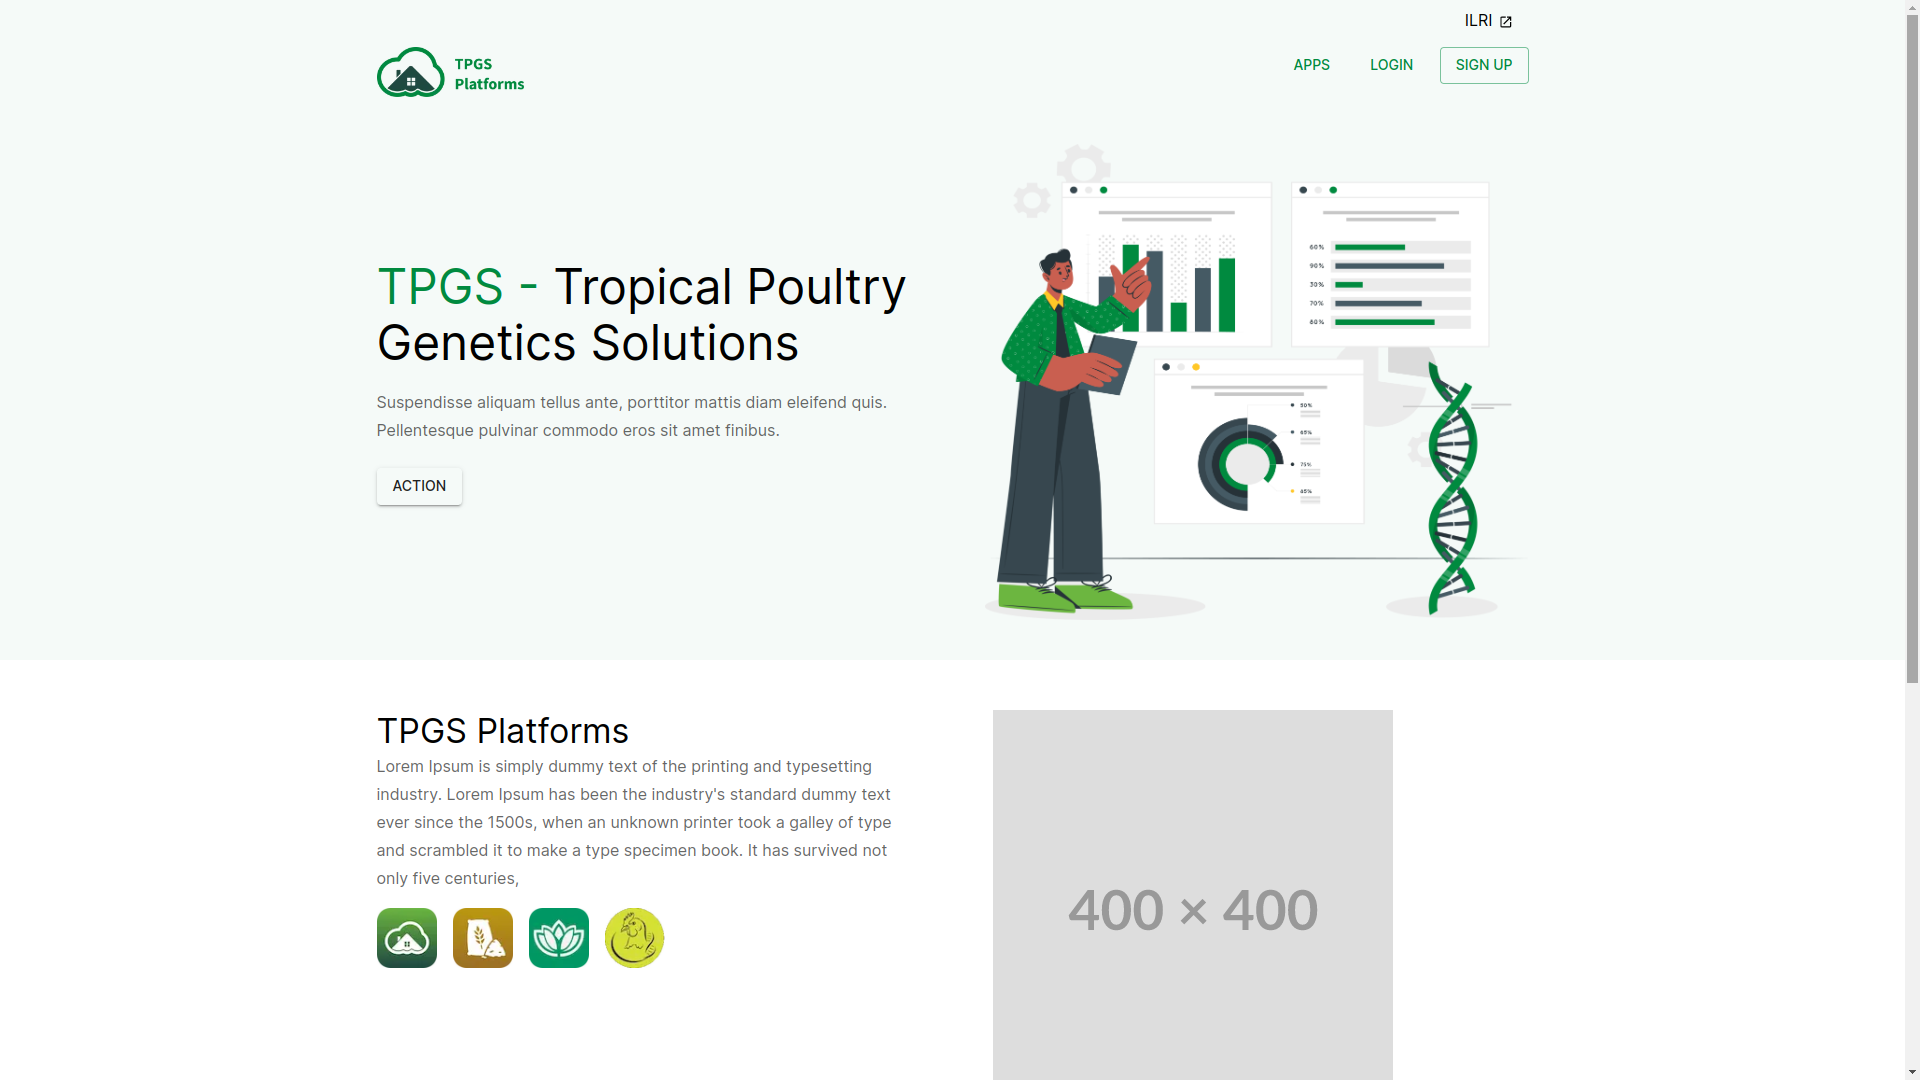
\includegraphics[width=20cm,keepaspectratio]{1.png}
\caption{TPGS platforms portal website}
\end{figure}

\pagebreak
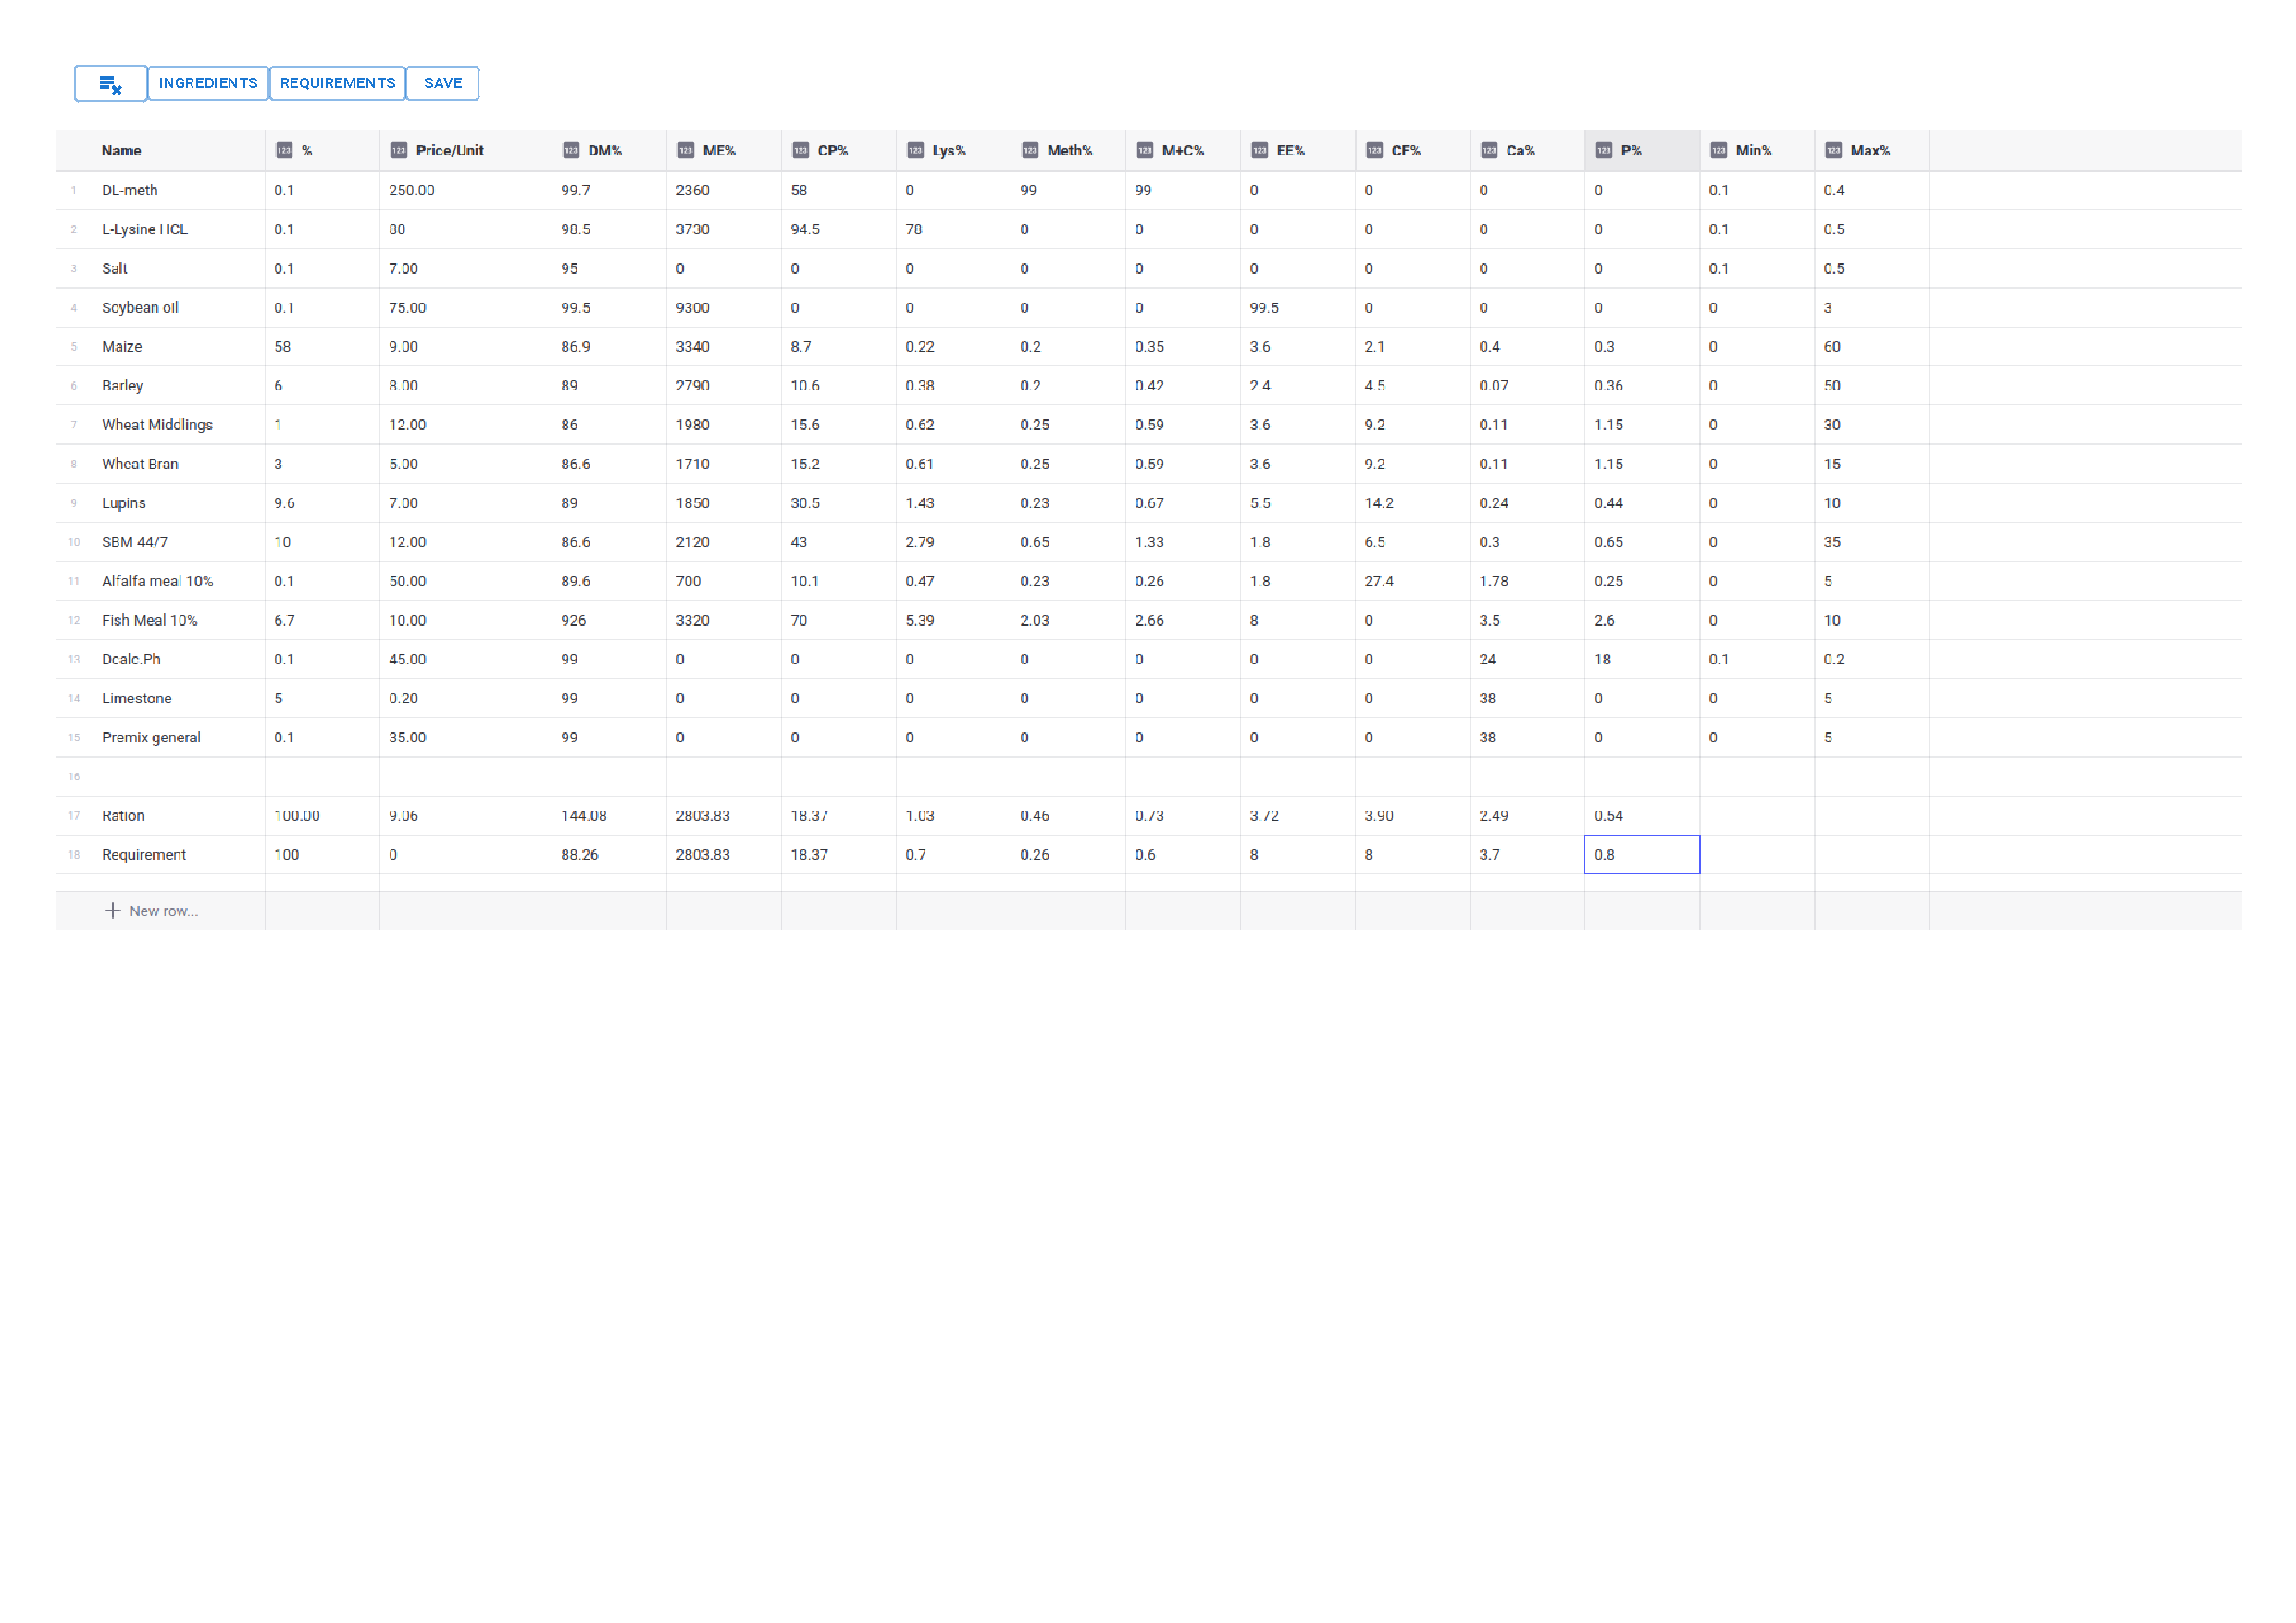
\includepdf[page=-, pagecommand={}]{feed_screen.pdf}
Feed Formulation
\end{document}